\newif\ifarxiv
%\arxivtrue

\ifarxiv
\documentclass[a4paper]{article}
\usepackage[top=1in, bottom=1.25in, left=1.25in, right=1.25in]{geometry}

\else
\documentclass[a4paper]{jpconf}

\fi

\usepackage{graphicx}
\usepackage{bm}        % for math
\usepackage{amssymb}   % for math
\usepackage{amsfonts}
\usepackage{amsmath}
\usepackage{epsfig}
\usepackage{units}
\usepackage{cite}
%\usepackage[numbers,square,sort&compress]{natbib}
\usepackage[utf8]{inputenc}
\usepackage[T1]{fontenc}
\usepackage{color}
\usepackage{hyperref}
%\usepackage{lineno}
%\linenumbers

%particles
\newcommand{\jpsi}{\rm J/$\psi$}
\newcommand{\psip}{$\psi^\prime$}
\newcommand{\jpsiDY}{\rm J/$\psi$\,/\,DY}
\newcommand{\chic}{$\chi_{\rm c}$}
\newcommand{\pip}{$\pi^{+}$}
\newcommand{\pim}{$\pi^{-}$}
\newcommand{\pizero}{$\pi^{0}$}
\newcommand{\kap}{K$^{+}$}
\newcommand{\kam}{K$^{-}$}
\newcommand{\pbar}{$\rm\overline{p}$}
\newcommand{\ccbar}{\ensuremath{\mathrm{c\overline{c}}}}
\newcommand{\bbbar}{\ensuremath{\mathrm{b\overline{b}}}}
\newcommand{\Dzero}{\ensuremath{\mathrm{D^{0}}}}
\newcommand{\Dzerobar}{\ensuremath{\mathrm{\overline{D}^{0}}}}
\newcommand{\Dpm}{\ensuremath{\mathrm{D^{\pm}}}}
\newcommand{\Ds}{\ensuremath{\mathrm{D_{s}^{\pm}}}}
\newcommand{\Dstar}{\ensuremath{\mathrm{D^{*\pm}}}}

%collision systems
\newcommand{\pp}{pp}
\newcommand{\pPb}{p--Pb}
\newcommand{\PbPb}{Pb--Pb}

%detectors
\newcommand{\ezdc}{$E_{\rm ZDC}$}

%units
\newcommand{\GeVc}{GeV/$c$}
\newcommand{\GeVcsq}{GeV/$c^2$}

%others
\newcommand{\degree}{$^{\rm o}$}
\newcommand{\s}{\ensuremath{\sqrt{s}}}
\newcommand{\snn}{\ensuremath{\sqrt{s_{\rm NN}}}}
\newcommand{\y}{\ensuremath{y}}
\newcommand{\pt}{\ensuremath{p_{\rm T}}}
\newcommand{\dedx}{d$E$/d$x$}
\newcommand{\dndy}{d$N$/d$y$}
\newcommand{\dndydpt}{${\rm d}^2N/({\rm d}y {\rm d}p_{\rm t})$}
\newcommand{\zpar}{\ensuremath{z_{||}}}
\newcommand{\zpargen}{\ensuremath{z_{||}^{\mathrm{part}}}}
\newcommand{\zpardet}{\ensuremath{z_{||}^{\mathrm{det}}}}
\newcommand{\ptchjet}{\ensuremath{p_{\mathrm{T,ch\, jet}}}}
\newcommand{\ptjet}{\ensuremath{p_{\mathrm{T,jet}}}}
\newcommand{\ptchjetgen}{\ensuremath{p_{\mathrm{T,ch\,jet}}^{\mathrm{truth}}}}
\newcommand{\ptchjetdet}{\ensuremath{p_{\mathrm{T,ch\,jet}}^{\mathrm{reco}}}}
\newcommand{\ptd}{\ensuremath{p_{\mathrm{T,D}}}}
\newcommand{\ptdgen}{\ensuremath{p_{\mathrm{T,D}}^{\mathrm{truth}}}}
\newcommand{\ptddet}{\ensuremath{p_{\mathrm{T,D}}^{\mathrm{reco}}}}
\newcommand{\antikt}{anti-\ensuremath{k_{\mathrm{T}}}}
\newcommand{\kt}{\ensuremath{k_{\mathrm{T}}}}
\newcommand{\pthard}{\ensuremath{p_{\mathrm{T,hard}}}}



\ifarxiv

\title{Measurement of D-meson tagged jets in pp collisions at $\s=7$~TeV with ALICE}
\date{}
\author{Salvatore Aiola, for the ALICE Collaboration \\
Physics Department, Yale University, New Haven, CT 06511\\
\href{mailto:salvatore.aiola@yale.edu}{salvatore.aiola@yale.edu}}
\begin{document}
\maketitle

\else

\begin{document}
\title{Measurement of D-meson tagged jets in pp collisions at $\s=7$~TeV with ALICE}
\author{Salvatore Aiola, for the ALICE Collaboration}
\address{Physics Department, Yale University, New Haven, CT 06511}
\ead{\href{mailto:salvatore.aiola@yale.edu}{salvatore.aiola@yale.edu}}

\fi




\begin{abstract}
We present the current status of the measurement of jets that contain a D meson (D-tagged jets) with \mbox{ALICE}.
D-meson candidates, identified via their hadronic decay channels, were combined with the other charged tracks reconstructed with the central tracking system, 
using the anti-$k_{\rm T}$ jet-finding algorithm.
The yield of D-tagged jets was extracted through an invariant mass analysis of the D-meson candidates.
A Monte Carlo simulation was used to determine the detector performance and validate the signal extraction techniques.
\end{abstract}

\section{Introduction}
At hadron colliders, charm quarks are produced as a result of a hard scattering of partons. Like lighter quarks or gluons, charm quarks
fragment into collimated sprays of hadrons called \emph{jets}. The charm content of the jet is conserved throughout the fragmentation process,
which is dominated by Quantum Chromo-Dynamics (QCD).
In the final state, the charm content can be identified by looking for the presence of charmed hadrons among the jet constituents.

The measurement of the charm jet production cross section in \pp\ collisions is a sensitive test of perturbative QCD (pQCD) calculations.
Heavy quarks are also an ideal probe of the Quark-Gluon Plasma (QGP)~\cite{STAR:2005a, PHENIX:2005a}
that is created in ultra-relativistic heavy-ion collisions. 
Hard scattered partons, including heavy quarks, interact with the QGP, which increases their virtuality and interferes with the
parton shower (\emph{jet quenching})~\cite{PHENIX:2008b, CMS:2012b, ALICE:2015a}.
At low parton energy, comparable to the charm mass, the charm quark is expected
to interact less strongly with the QGP~\cite{Dokshitzer:2001}, when compared to light quarks and gluons.

Most of the charm measurements performed so far at the LHC report the production cross section of hadrons
containing heavy quarks~\cite{ALICE:2012d, LHCb:2013a, ATLAS:2016a, ALICE:2016b}.
Measuring the kinematic observables of jets with charm content implies integrating out some of the hadronization degrees of freedom. 
Since hadronization is a highly non-perturbative process, known only with large uncertainties~\cite{dEnterria:2014}, 
using observables less dependent on this process may improve comparisons with pQCD calculations.
Furthermore, the measurement of the fragmentation function (FF) of charmed hadrons 
can provide important insights into the charm production mechanism~\cite{CDF:1990, UA1:1990, STAR:2009a}.
ATLAS has measured the FF of \Dstar\ mesons, observing a large discrepancy with Monte Carlo
event generators~\cite{ATLAS:2012d}. ALICE has the potential to extend this measurement to low $z$, where $z$ is the fraction
of jet momentum carried by the D meson.

\section{The ALICE Experiment}
ALICE is the experiment dedicated to the study of heavy-ion collisions at the LHC.
The central barrel detectors ($\lvert \eta\rvert \lesssim 1$) are located inside a large solenoid magnet, providing a
field $B = 0.5$~T.
%, parallel to the beam line.
The \emph{Inner Tracking System} (ITS) is a six-layer silicon detector that allows a precise determination of the primary vertex 
and of displaced secondary vertices of weak decays.
The main tracking detector is the \emph{Time Projection Chamber} (TPC), which, combined with the ITS, allows reconstruction of tracks 
from low ($\pT\approx0.15$~\GeVc) to high transverse momentum
($\pT\approx100$~\GeVc) with good momentum resolution and tracking efficiency.
Several detectors contribute to the Particle Identification (PID) capabilities of ALICE. 
In this analysis we use the \dedx\ measurement from the TPC and
the velocity $\beta$ of the particles measured by the \emph{Time Of Flight} (TOF) detector,
an array of Multigap Resistive Plate Chambers (MRPC).
A full description of ALICE and of its performance during LHC Run-1 is available at Ref.~\cite{ALICE:2014b}.

\section{Analysis procedures}
The analysis relies on the well-established D meson reconstruction techniques~\cite{ALICE:2012d, ALICE:2016a}, as well as
jet reconstruction methods~\cite{ALICE:2013c, ALICE:2015a, ALICE:2015e}, both developed by the ALICE Collaboration during Run-1.

%\subsection{\Dzero-jet reconstruction}
For this study, only charged tracks were used to reconstructed the jets (\emph{charged jets}).
Track quality cuts were applied to ensure good momentum resolution. 
Decay products of the D mesons were found among reconstructed tracks with the best momentum resolution, which entails at least one space
point in one of the two layers of the ITS closest to the beam pipe.
For jet reconstruction, this last requirement was lifted to achieve a more uniform azimuthal acceptance.

\Dzero\ mesons ($m=1.865$~\GeVcsq, $c\tau=123\,\mu$m) and their charge conjugates were used to tag jets with charm content.
They were reconstructed via their hadronic decay: \Dzero $\rightarrow$ \pip \kam (BR = 3.88\%)~\cite{PDG:2014}. 
The topological cuts select unlike-sign (US) pairs that form a secondary vertex displaced from the reconstructed
primary vertex. PID on the \Dzero\ candidate daughters was used to reject pairs not compatible with the $\pi$K hypothesis.
%When available, PID was used also to assign mass values to the \Dzero\ candidate daughters, otherwise
%the pair was used twice, once with each mass combinations (\pip \kam and \pim \kap). 
The four-momenta of each \Dzero\ candidate and all reconstructed tracks
(excluding the two daughters of the \Dzero) were used as input to the \antikt\ jet-finding algorithm~\cite{Cacciari:2008c}.
Only jets containing the \Dzero\ candidates were retained.

%\subsection{Invariant mass analysis}
%\Dzero\ candidates and their associated jets are sorted according to jet momentum, \Dzero\ momentum and jet momentum
%fraction carried by the \Dzero.
In order to extract the signal out of the combinatorial background,
three different invariant mass analysis techniques were developed and their performance compared.
\begin{description}
%\subsubsection*{Invariant mass fit}
\item[Invariant mass fit]
%The \Dzero-jet candidates are divided in bins of the transverse momentum of their associated jet (\ptchjet) and 
The invariant mass distribution of the \Dzero\ candidates was constructed for various intervals of their associated-jet transverse momentum (\ptchjet);
each candidate was given a weight corresponding to the inverse of its reconstruction efficiency $\epsilon(\ptd)$.
The invariant mass distribution was fit using the sum of an exponential function (background) and a Gaussian (signal). 
The \Dzero-jet yield $N^{\rm \Dzero\hbox{-}jet}(\ptchjet)$ was extracted from
the fit parameters.
%\subsubsection*{Side-band subtraction}
\item[Side-band subtraction]
For each \ptd\ interval, the \Dzero-jet yield $N^{\rm \Dzero\hbox{-}jet}(\ptchjet,\ptd)$ was extracted by subtracting the
\ptchjet\ distribution in the side bands of the invariant mass distribution ($4\sigma_{\rm fit} < \lvert m - m_{\rm fit} \rvert < 8\sigma_{\rm fit}$) 
from the \ptchjet\ distribution in the peak area ($\lvert m - m_{\rm fit} \rvert < 2\sigma_{\rm fit}$); the peak position $m_{\rm fit}$, peak width $\sigma_{\rm fit}$ and side-band normalization factor were extracted 
by fitting the invariant mass distribution with an exponential + Gaussian function; the \ptd\ bins were weighted by the inverse of the \Dzero-meson reconstruction efficiency $\epsilon(\ptd)$ and summed over:
\begin{equation*}
N^{\rm \Dzero\hbox{-}jet}(\ptchjet)=\sum_{\ptd} \frac{1}{\epsilon(\ptd)} 
\left[N_{\rm peak}^{\rm \Dzero\hbox{-}jet}(\ptchjet,\ptd) - 
\frac{B_{\rm peak}^{\rm fit}}{B_{\rm SB}} 
N_{\rm SB}^{\rm \Dzero\hbox{-}jet}(\ptchjet,\ptd)\right],
\end{equation*}
where $B_{\rm peak}^{\rm fit}$ and $B_{\rm SB}$ are respectively the total background
in the peak area estimated by fitting the invariant mass distribution and the total
background in the side bands.

%\subsubsection*{Like-sign subtraction}
\item[Like-sign subtraction]
This method is analogous to the side-band method. In this case the background \ptchjet\ distribution was provided by the like-sign (LS) $\pi$K pairs and
subtracted from the corresponding unlike-sign (US) pairs:
\begin{equation*}
N^{\rm \Dzero\hbox{-}jet}(\ptchjet)=\sum_{\ptd} \frac{1}{\epsilon(\ptd)} 
\left[N_{\rm US, peak}^{\rm \Dzero\hbox{-}jet}(\ptchjet,\ptd) - 
\frac{B_{\rm US, SB}}{B_{\rm LS, SB}} 
N_{\rm LS, peak}^{\rm \Dzero\hbox{-}jet}(\ptchjet,\ptd)\right],
\end{equation*}
where $B_{\rm US, SB}$ and $B_{\rm LS, SB}$ are respectively the integral of
the side bands in the US and in the LS invariant mass distributions.
\end{description}
%\subsection{Monte Carlo simulations}
Monte Carlo (MC) simulations were used to determine the detector performance and validate the analysis techniques.
PYTHIA6 (6.4.25)\cite{Sjostrand:2006} (tune Perugia-2011) was used 
%as event generator.
%In the \emph{minimum-bias} production, PYTHIA is configured to provide minimum-bias (MB) 
to provide \pp\ collision events at $\s=7$~TeV.
%In the \emph{charm-enhanced} production PYTHIA is configured to retain only events with a \ccbar\ pair 
%with a cut on the minimum \pT\ of the hard scattered parton.
Particles produced by PYTHIA were propagated through the detector using the GEANT3 transport code~\cite{GEANT3-url}.

\section{Results}
\label{sect:detperf}
\begin{figure}[tb]
\centering
\begin{minipage}{.48\textwidth}
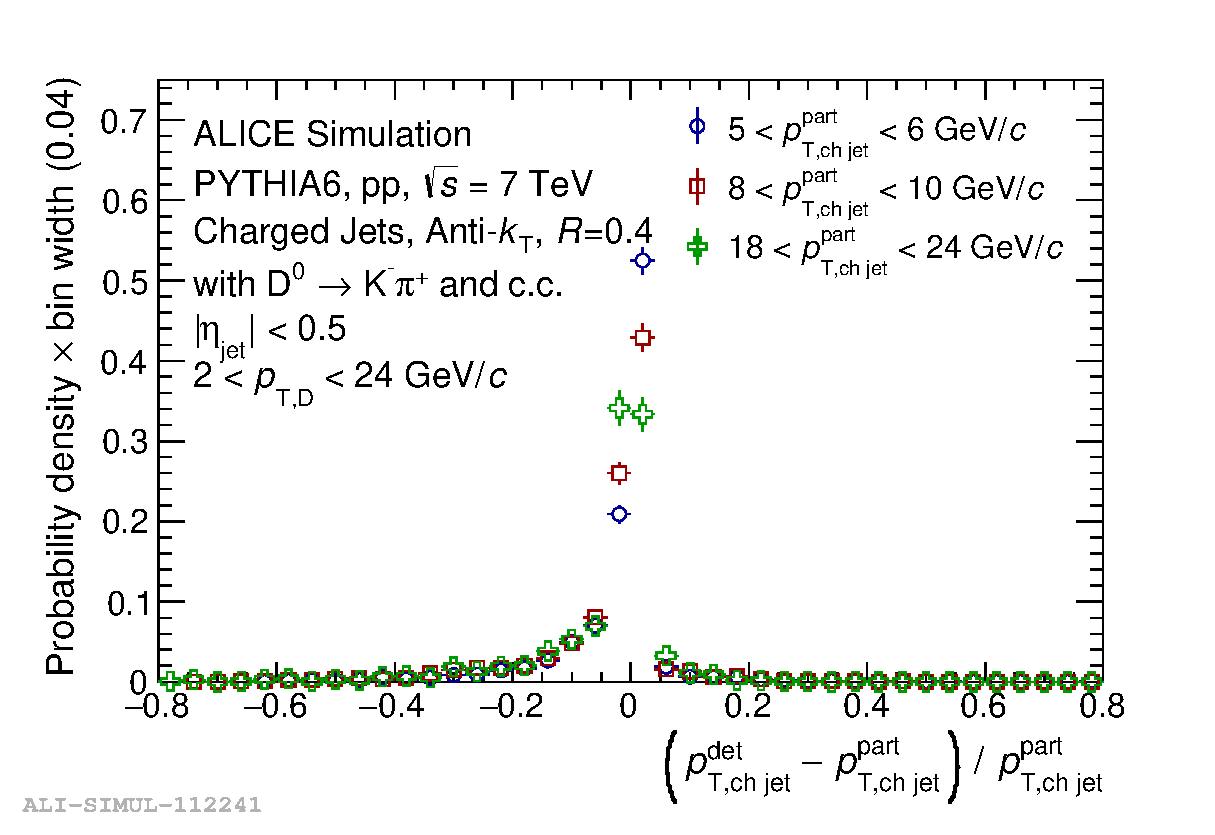
\includegraphics[width=\textwidth]{img/HQ16_Simulation_DetectorResponse}
\caption{\label{fig:HQ16_Simulation_DetectorResponse} Probability density distribution of the jet momentum shift in \ptchjet\ intervals.}
\end{minipage}\hspace{1pc}%
\begin{minipage}{.48\textwidth}
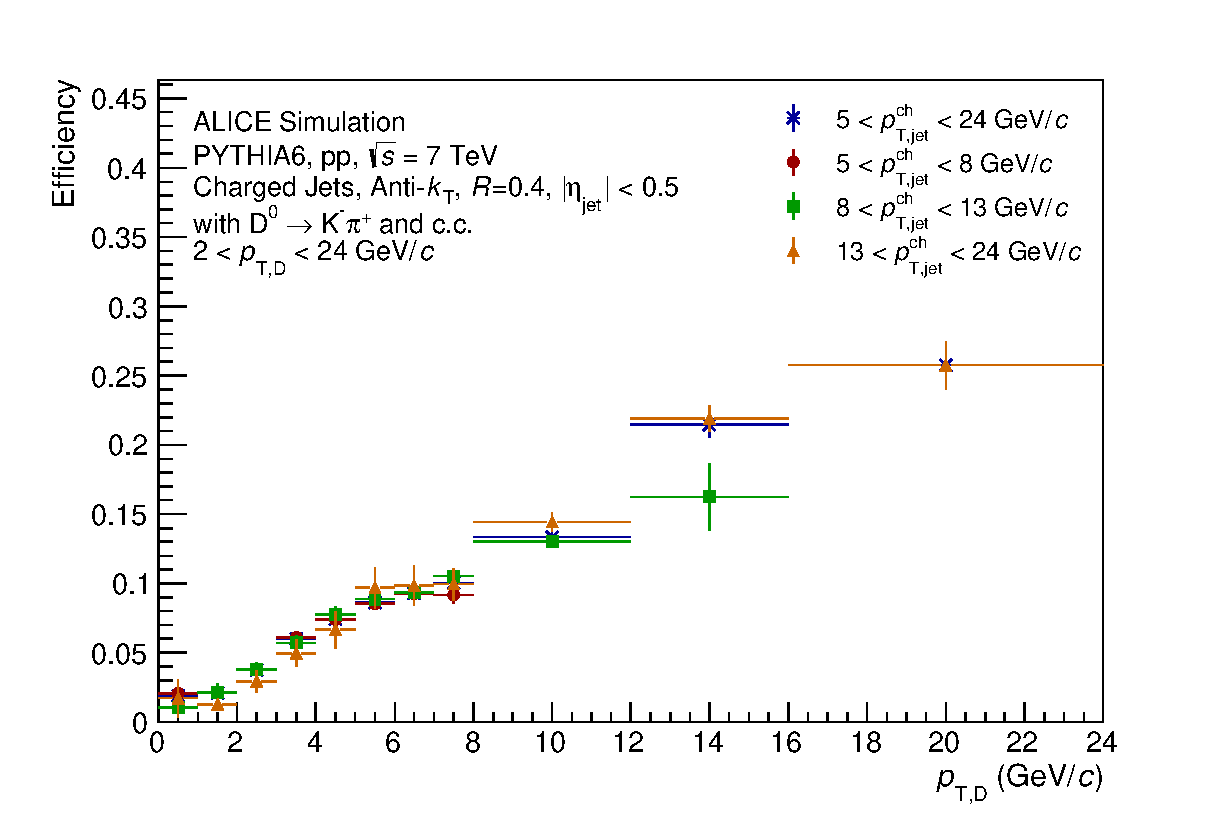
\includegraphics[width=\textwidth]{img/HQ16_Simulation_EfficiencyVsDPt}
\caption{\label{fig:HQ16_Simulation_EfficiencyVsDPt}Efficiency~$\times$~Acceptance of \Dzero\ mesons vs. \ptd\ in \ptchjet\ inetrvals.}
\end{minipage} 
\end{figure}
\ifarxiv
\begin{figure}[tb]
\centering
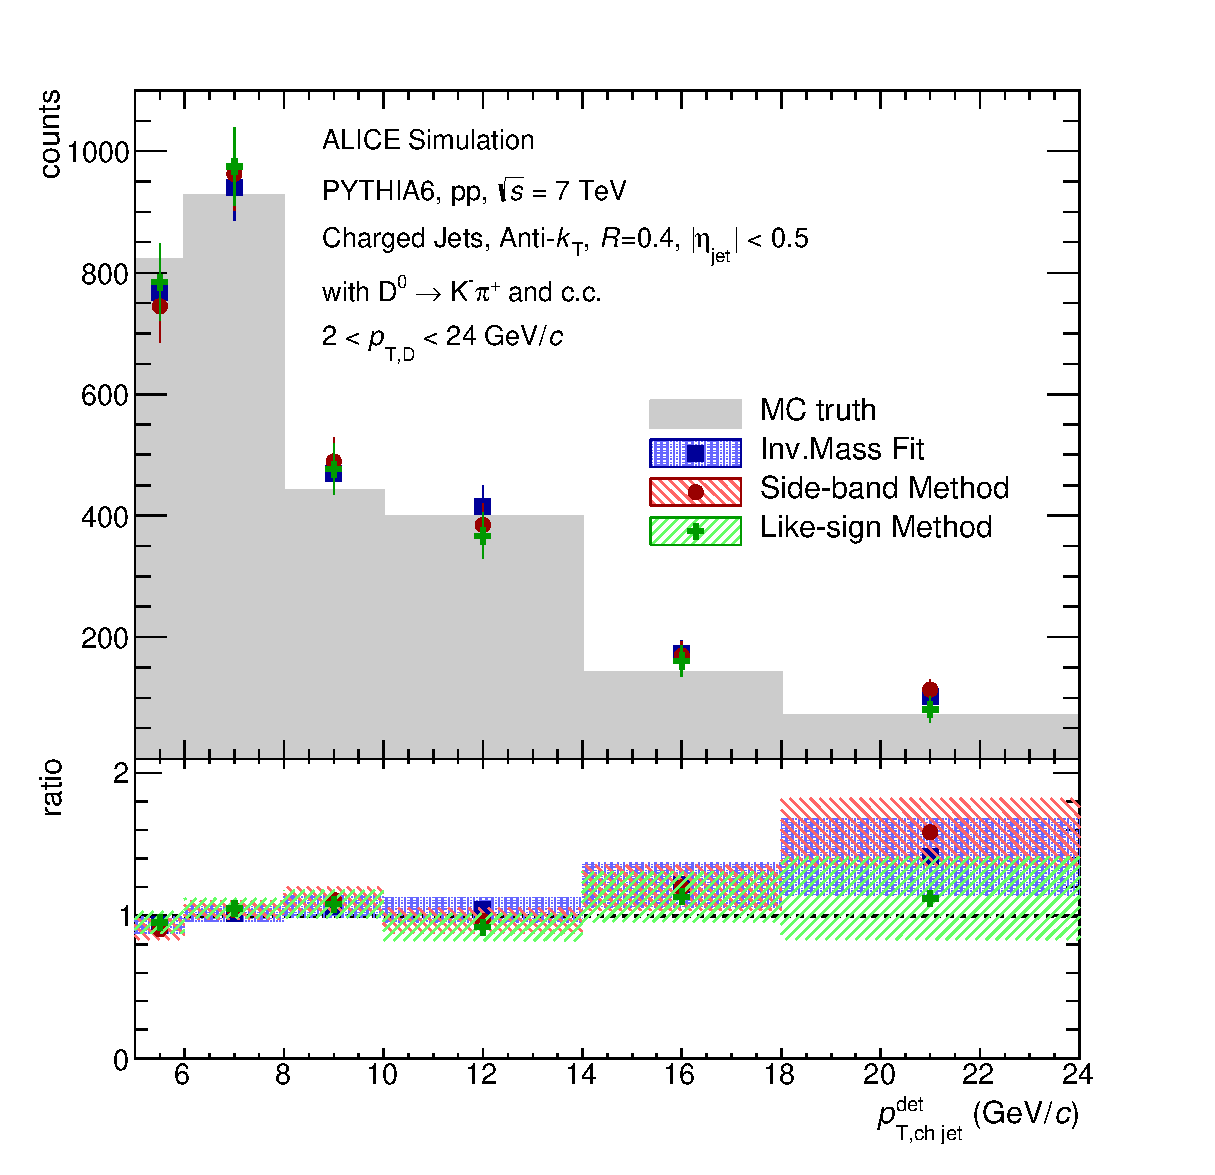
\includegraphics[width=.50\textwidth]{img/HQ16_Simulation_MethodComparison}\hspace{1pc}%
\caption{\label{fig:HQ16_Simulation_MethodComparison}\Dzero-jet signal yield extracted using the invariant mass fit (blue squares), side-band method (red circles) and like-sign method (green triangles)
compared with the MC truth (gray filled area). The bottom panel shows the ratio to the MC truth. The yields are corrected for the reconstruction efficiency but not for distortions due to detector jet-momentum resolution.}
\end{figure}
\fi
%The detector performance was assessed using the charm-enhanced MC production. 
In order to determine the detector performance, reconstructed detector-level D-tagged jets were matched with their corresponding counterparts at generator-level.
The variable
%\begin{equation}
$\delta_{\ptchjet}=\left( \ptchjetdet - \ptchjetgen \right) / \ptchjetgen$,
%\label{eq:energyshift}
%\end{equation}
was computed for each matched pair,
where \ptchjetdet\ and \ptchjetgen\ are the transverse momenta of the D-tagged jet at detector-level and at generator-level, respectively.
Its probability density distribution is shown in Fig.~\ref{fig:HQ16_Simulation_DetectorResponse} for three \ptchjetgen\ intervals. No significant dependence on \ptchjetgen\ was observed.
The shape of the distribution features a sharp peak at zero and is skewed towards negative values, due to tracking inefficiency (higher probability of
reconstructing smaller jet momenta than the generated ones). The jet momentum resolution (standard deviation of $\delta_{\ptchjet}$) for \Dzero-tagged jets is approximately \mbox{$11$\%}, 
slightly smaller with respect to its value for inclusive jets~\cite{ALICE:2015e}. The mean jet momentum shift is approximately \mbox{$-3$\%}.
The reconstruction efficiency is calculated as the ratio of the yield of reconstructed D-tagged jets over all generated D-tagged jets, as a function of generator-level observables.
It is shown in Fig.~\ref{fig:HQ16_Simulation_EfficiencyVsDPt} as a function of \ptd\ for different \ptchjet\ intervals; it shows a strong dependence on \ptd, mainly due to
varying topological cuts. No significant dependence on \ptchjet\ is observed in the interval $5<\ptchjet<24$~\GeVc.
%The minimum-bias production was used to validate the invariant mass analysis. 
Figure~\ref{fig:HQ16_Simulation_MethodComparison} shows the D-tagged jet yields as a function of \ptchjetdet\ obtained using the invariant mass fit, 
side-band and like-sign methods, compared to the MC truth. All signal extraction methods perform well and do not show significant biases, beyond the statistical uncertainties assigned to each.
\ifarxiv
\else
\begin{figure}[tb]
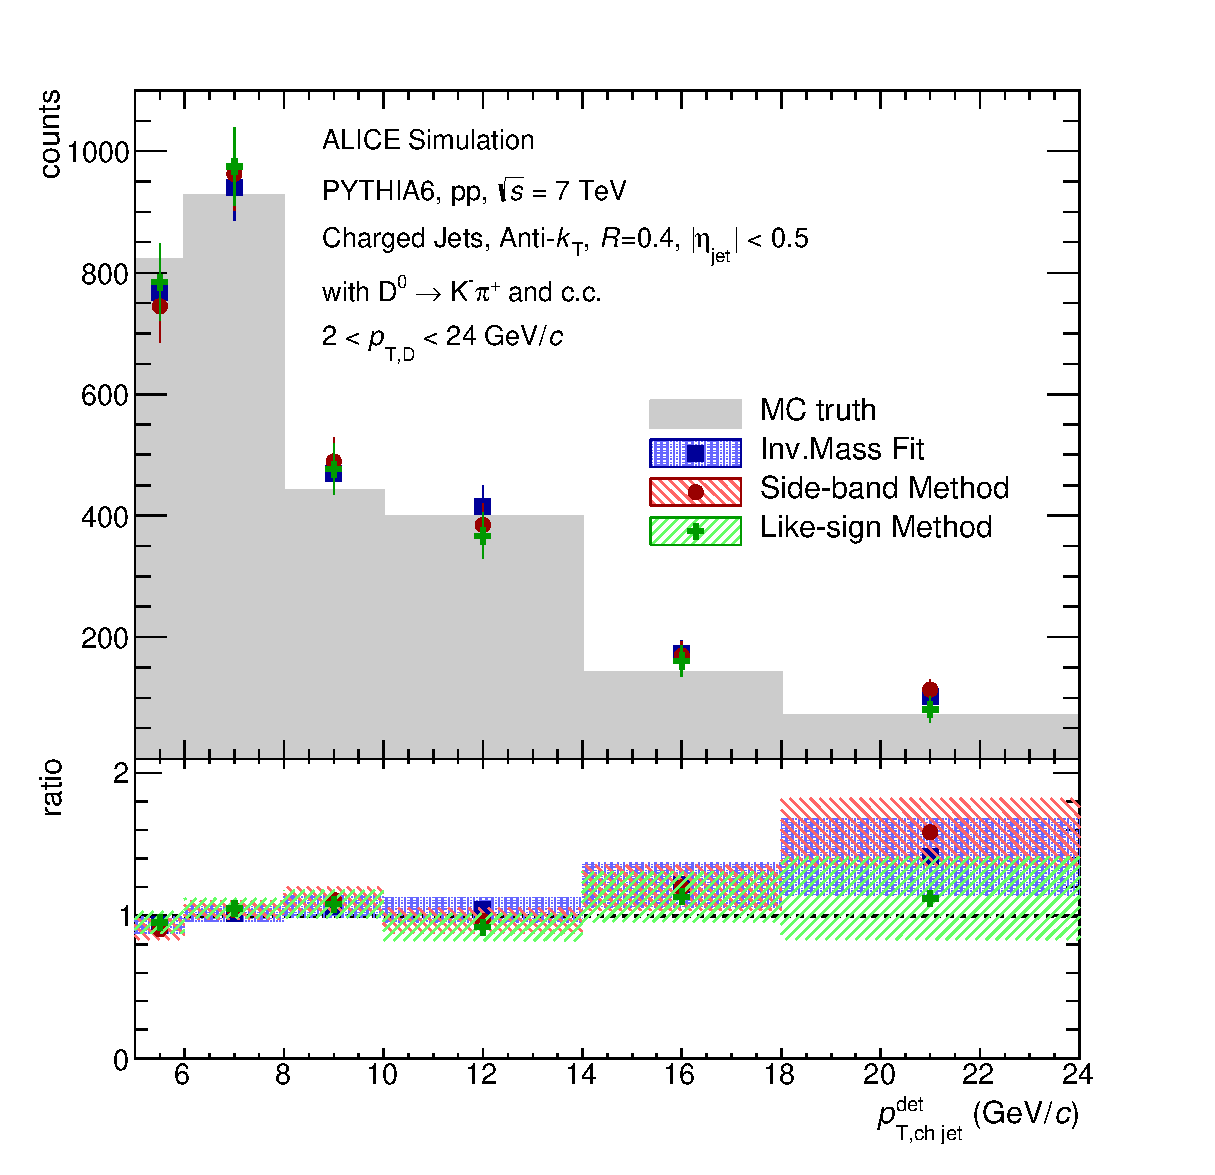
\includegraphics[width=.50\textwidth]{img/HQ16_Simulation_MethodComparison}\hspace{1pc}%
\begin{minipage}[b]{.50\textwidth}\caption{\label{fig:HQ16_Simulation_MethodComparison}\Dzero-jet signal yield extracted using the invariant mass fit (blue squares), side-band method (red circles) and like-sign method (green triangles)
compared with the MC truth (gray filled area). The bottom panel shows the ratio to the MC truth. The yields are corrected for the reconstruction efficiency but not for distortions due to detector jet-momentum resolution.}
\end{minipage}
\end{figure}
\fi
\section{Conclusions}
ALICE has the potential for measuring jets with charm content tagged using reconstructed D mesons.
%in pp collisions, especially at low momentum ($\ptchjet \lesssim 30$~\GeVc) with the data collected at $\s=7$~TeV,
%as well as the intermediate jet momentum ($\ptjet\approx100$~\GeVc) and
%low D-meson momentum by exploiting the data collected at $\s=8,\,13$~TeV with the calorimeter triggers.
%In \PbPb\ and \pPb\ collisions ALICE will study cold and hot nuclear matter effects
%looking at the yields and fragmentation functions of \Dzero-tagged jets.
The ALICE detector performance for \Dzero-tagged jets was assessed using MC simulations
for pp collisions at $\s=7$~TeV. The \Dzero-jet momentum resolution was determined to be about 11\%; the reconstruction efficiency, independent of \ptchjet, ranges from 5\% to 25\% as a function of \ptd.
Three methods were implemented to extract the signal: invariant mass fit, side-band and like-sign subtraction.
The three methods were validated using a MC simulation and do not show biases larger than the statistical uncertainties.

\ifarxiv
\else
\section*{References}
\fi
\bibliography{biblio}{}
\bibliographystyle{iopart-num}

\end{document}


